% !TeX root = ../main.tex
\section{Đội ngũ}

\subsection{Danh sách và vai trò thành viên}

Vai trò làm việc dự kiến của từng thành viên trong nhóm được chia thành 2 phần việc chính: Business and Development responsibility.

Với Business responsibility bao gồm các công việc sau được chia cho từng cá nhân dưới đây.

\vspace{0.25cm}
\begin{tabular}{l l l}
\toprule
\textbf{Họ và Tên} & \textbf{MSSV} & \textbf{Business responsibility} \\
\midrule
23127141 & Trần Cao Vân & Project manager, Business analyst \\
23127318 & Lê Hồ Đan Anh & Business analyst \\
23127016 & Lưu Huy Minh Quang & Project owner \\
23127404 & Lê Tuấn Lộc & Marketing \\
23127465 & Nguyễn Hồ Anh Quốc & Finance\\
\bottomrule
\end{tabular}
\vspace{0.5cm}


Với Research \& Development sẽ các công việc sau:

\vspace{0.25cm}
\begin{tabular}{l l l}
\toprule
\textbf{Họ và Tên} & \textbf{MSSV} & \textbf{R\&D responsibility} \\
\midrule
23127141 & Trần Cao Vân & Frontend head, Tester \\
23127318 & Lê Hồ Đan Anh & Backend developer \\
23127016 & Lưu Huy Minh Quang & Backend developer \\
23127404 & Lê Tuấn Lộc & Backend head \\
23127465 & Nguyễn Hồ Anh Quốc & Frontend developer\\
\bottomrule
\end{tabular}
\vspace{0.5cm}


\subsection{Năng lực kinh nghiệm}

Chi tiết năng lực, kinh nghiệm và các kỹ năng của từng thành viên liên quan đến dự án Start up.

\begin{itemize}
    \item Trần Cao Vân:
    \begin{itemize}
        \item Kinh nghiệm: 
        \begin{itemize}
            \item Tham gia tổ chức sự kiện cho khoa
            \item Tham gia các cuộc thi làm business plan liên quan đến công nghệ, AI, 
            \item Quản lý và vận hành nhóm, các cuộc thi.
        \end{itemize}
        \item Kỹ năng: 
        \begin{itemize}
            \item Lập trình web \& app
            \item Các kĩ năng sử dụng LLM, Machine Learning.
            \item Làm business plan 
            \item Quản lý hoạt động nhóm.
        \end{itemize}
        \item Điểm yếu: 
        \begin{itemize}
            \item Khả năng kiểm soát thời gian chưa vững, 
            \item Không có nhiều kinh nghiệm về các mảng kinh tế, quản lý tài chính.
            \item Khả năng tiếp cận các công nghệ mói còn chậm
        \end{itemize}
    \end{itemize}

    \item Lê Hồ Đan Anh:
    \begin{itemize}
        \item Kinh nghiệm:
            \begin{itemize}
                \item Quản lý và điều phối nhóm trong các dự án và cuộc thi cả học thuật và hackathon.
                \item Phân tích nghiệp vụ, thiết kế hệ thống và phát triển phần mềm trong các đồ án
                \item Hỗ trợ CLB các cuộc thi liên quan đến ý tưởng, hackathon.
            \end{itemize}
        \item Kỹ năng:
            \begin{itemize}
                \item Lập trình web/app
                \item Phân tích nghiệp vụ
                \item Phân tích và thiết kế hệ thống thông tin, thiết kế cơ sở dữ liệu
                \item Quản lý và điều phối nhóm
                \item Git, GitHub và làm việc theo quy trình phát triển phần mềm
                \item Giải quyết vấn đề và tư duy logic
            \end{itemize}
        \item Điểm yếu:
            \begin{itemize}
                \item Chưa được đào tạo chuyên sâu về các lĩnh vực kinh doanh như marketing và finance
                \item Kinh nghiệm thực tế trong các dự án quy mô doanh nghiệp còn hạn chế
            \end{itemize}
    \end{itemize}

    \item Nguyễn Hồ Anh Quốc:
    \begin{itemize}
        \item Kinh nghiệm:
            \begin{itemize}
                \item Tham gia các dự án phát triển phần mềm trong các đồ án môn học
                \item Tham gia các cuộc thi nhỏ của trường về ý tưởng sinh viên
            \end{itemize}
        \item Kỹ năng:
            \begin{itemize}
                \item Lập trình web \& app
                \item Kiến thức nền tảng về an toàn thông tin, bảo mật và mã hóa
                \item Thiết kế cơ sở dữ liệu và quản lý dữ liệu
                \item Sử dụng Git/GitHub để quản lý phiên bản mã nguồn
                \item Tư duy logic, giải quyết vấn đề và làm việc nhóm
            \end{itemize}
        \item Điểm yếu:
            \begin{itemize}
                \item Chưa có kinh nghiệm thực tập hoặc làm việc trong môi trường doanh nghiệp
                \item Kinh nghiệm về kinh doanh, marketing và quản lý sản phẩm còn hạn chế
                \item Cần cải thiện kỹ năng giao tiếp và thuyết trình
                \item Cần cải thiện sự tự tin, tính chủ động và khả năng đưa ra ý kiến trong quá trình làm việc nhóm
            \end{itemize}
    \end{itemize}

    \item Lưu Huy Minh Quang:
    \begin{itemize}
        \item Kinh nghiệm:
            \begin{itemize}
                \item Trải qua nhiều các dự án liên quan đến Lập trình web.
                \item Đã từng có web đưa ra hoạt động thực tế (quy mô nhỏ).
                \item Tham gia các sự kiện liên quan đến gaming, nắm rõ phần cứng và thị trường liên quan
                \item Hỗ trợ tổ chức các hoạt động trải nghiệm của lớp.
            \end{itemize}
        \item Kỹ năng:
            \begin{itemize}
                \item Lập trình web/app.
                \item Thiết kế hệ thống, cơ sở dữ liệu.
                \item Sử dụng Git/GitHub để quản lý phiên bản mã nguồn.
                \item CI/CD, triển khai hệ thống.
                \item Tư duy logic, giải quyết vấn đề và làm việc nhóm.
            \end{itemize}
        \item Điểm yếu:
            \begin{itemize}
                \item Dễ bị lung lay bởi các yếu tố bên ngoài.
                \item Chưa có kiến thức đủ sâu về Marketing.
                \item Kinh nghiệm thực tế trong môi trường doanh nghiệp còn hạn chế.
            \end{itemize}
    \end{itemize}
    
    \item Lê Tuấn Lộc:
    \begin{itemize}
        \item Kinh nghiệm:
            \begin{itemize}
                \item Tham gia phát triển các dự án web Fullstack trong các đồ án môn học.
                \item Thiết kế, phát triển RESTful APIs và xây dựng cơ sở dữ liệu.
                \item Tích hợp các dịch vụ bên thứ ba (thanh toán, xác thực người dùng).
                \item Triển khai thử nghiệm các ứng dụng web lên các nền tảng đám mây (Vercel, Render).
                \item Tham gia các cuộc thi của trường liên quan đến hackathon, xây dựng dự án.
            \end{itemize}
        \item Kỹ năng:
            \begin{itemize}
                \item Lập trình web (React/NextJS, Node.js/Java).
                \item Sử dụng Git/GitHub để quản lý mã nguồn và làm việc nhóm.
                \item Thiết kế cơ sở dữ liệu và xây dựng API.
                \item Tư duy logic, giải quyết vấn đề và tự học công nghệ mới.
                \item Thiết kế giao diện người dùng (UI/UX) cơ bản.
            \end{itemize}
        \item Điểm yếu:
            \begin{itemize}
                \item Thiếu kinh nghiệm làm việc trong môi trường doanh nghiệp thực tế.
                \item Chưa có nhiều kiến thức về marketing và quản lý tài chính.
                \item Quản lý và phân bổ thời gian đôi lúc chưa tối ưu khi xử lý nhiều đầu việc cùng lúc.
            \end{itemize}
    \end{itemize}
    
\end{itemize}

\subsection{Lý do đội ngũ phù hợp để triển khai ý tưởng}

Các thành viên trong nhóm đều là sinh viên năm 3, đã làm quen với quy trình làm việc R\&D để thực hiện sản phẩm phần mềm nên việc thiết kế cũng phù hợp. Có vài thành viên đã từng tham gia các cuộc thi, đóng vai trò là nhóm trưởng và từng thực hiện các business plan liên quan ít nhiều đến kinh tế. Bên cạnh đó, ý tưởng liên quan đến gaming gear cũng phù hợp với sinh viên trong ngành công nghệ thông tin. Đội ngũ này dễ dàng tiếp cận và tìm hiểu các thông tin thị trường hơn và cơ bản nắm được nhu cầu của giới trẻ sử dụng gaming gear.

Bên cạnh nền tảng kỹ thuật, các thành viên trong nhóm đều có niềm yêu thích đối với gaming gear và thường xuyên theo dõi các sản phẩm, xu hướng cũng như cộng đồng công nghệ. Nhóm nhận thấy nhiều người, đặc biệt là học sinh, sinh viên và người mới trải nghiệm, có nhu cầu sử dụng các thiết bị chất lượng nhưng gặp rào cản về chi phí sở hữu. Từ đó hình thành mong muốn xây dựng một nền tảng không chỉ hỗ trợ việc thuê và cho thuê gaming gear một cách thuận tiện, mà còn phát triển thành một cộng đồng nơi người dùng có thể chia sẻ trải nghiệm, đánh giá thiết bị, kết nối với các cửa hàng và những người có cùng sở thích. Việc xuất phát từ nhu cầu thực tế và sự am hiểu về lĩnh vực giúp nhóm dễ dàng tiếp cận thị trường mục tiêu, thấu hiểu hành vi người dùng và đề xuất những tính năng phù hợp.

Tuy nhiên bên cạnh đó, với việc thiếu kinh nghiệm liên quan đến kinh tế và thực sự tham gia vào các doanh nghiệp start up, các công ty. Vậy nên cần thiết có những người hỗ trợ về mặt kiến thức, những kinh nghiệm nhóm chưa có. Vậy nên vẫn có khả năng sẽ tìm hiểu những sự hỗ trợ sao cho đảm bảo khả năng thực hiện của startup.

\subsection{Cơ cấu tổ chức}

Với số lượng thành viên nhỏ, nhóm quyết định startup sẽ có cơ cấu tổ chức dưới 2 hình thức: business responsibility và R\&D responsibility. Với việc mỗi thành viên đảm nhiệm đồng thời cả 2 vai trò trên. 

Sơ đồ tổ chức giữa các thành viên nhóm như sau:

\begin{figure}[H]
    \centering
    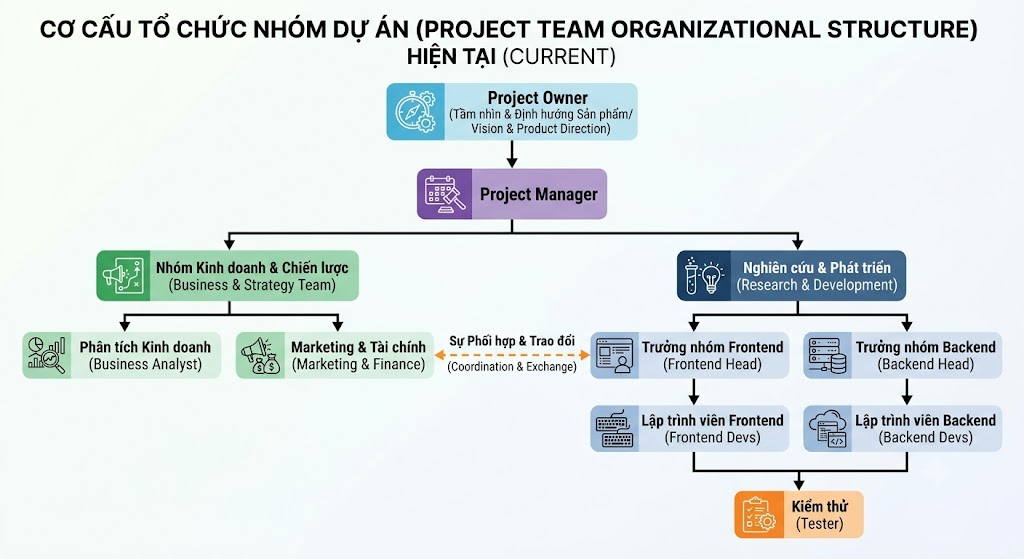
\includegraphics[width=0.75\linewidth]{../PA1/figures/organization.png}
    \caption{Sơ đồ thể hiện cơ cấu tổ chức của nhóm Start Up}
    \label{fig:my_unique_label}
\end{figure}


Mỗi thành viên đều đảm nhận một vai trò liên quan đến business, các vài trò được chia như sau phù hợp với khả năng và nguyện vọng mỗi người:

\begin{itemize}

  \item \textbf{Project manager:} quản lý quá trình hoạt động của nhóm, phân chia công việc cho các thành viên, theo dõi tiến độ của các thành viên, và tổ chức các cuộc họp nhóm.
  \item \textbf{Project owner:} định hướng tầm nhìn của sản phẩm, đảm bảo sản phẩm đáp ứng đúng mục tiêu. Hỗ trợ đưa ra các quyết định chiến lược và xác định các tính năng cần ưu tiên.
  \item \textbf{Business analyst:} Phân tích nhu cầu thị trường, khảo sát thị trường, xây dựng yêu cầu nghiệp vụ, phân tích thị trường và các đối thủ, đề xuất giải pháp kinh doanh.
  \item \textbf{Marketing:} Xây dựng chiến lược marketing và lập kế hoạch truyền thông. Xác định các kênh quảng bá và các đối tác có thể thực hiện marketing. Xác định khách hàng mục tiêu, ICP.
  \item \textbf{Finance:} Quản lý ngân sách dự án, theo dõi chi phí. Phân tích doanh thu và lợi nhuận, đánh giá tính khả thi về mặt tài chính cho startup. Lập kế hoạch tài chính.
\end{itemize}

Research \& Development sẽ chia thành 2 bộ phận là Frontend và Backend, vị trí của mỗi người được chia theo khả năng và kinh nghiệm làm việc. Bộ phận chịu trách nhiệm về việc phát triển sản phẩm

\begin{itemize}
  \item \textbf{Frontend head}: Phụ trách quản lý, định hướng chính cho UI/UX, thiết kế và triển khai các component, page, và các chức năng của front end. Review code
  \item \textbf{Frontend developer}: Thiết kế và triển khai các component, page. Kết nối API, kiểm thử, sửa lỗi. 
  \item \textbf{Backend head}: Phụ trách quản lý, định hướng chính cho các API, database. Review code, định hướng kỹ thuật Backend. 
  \item \textbf{Backend developer}: Xây dựng API và thiết kế database. Viết business tương ứng và API usage guide. Kiểm thử, sửa lỗi nếu cótechnical development .
  \item \textbf{Tester}: Thực hiện Functional Testing, viết test case phù hợp.
\end{itemize}

Các công việc được bàn với nhau qua các buổi họp và từng thành viên sẽ được chia công việc với nhau.

Với các công việc R\&D, trưởng bộ phận sẽ đảm nhận trách nhiệm chính để chia công việc với nhau, kiểm tra chất lượng và đảm bảo khả năng thực hiện. 

Khi công việc của bộ phận hoàn thành, trưởng bộ phận chịu trách nhiệm cao nhất và đầu tiên cho các lỗi xảy ra rồi tiếp đến là thành viên thực hiện.


\subsection{Vị trí, năng lực còn thiếu}
Các vị trí của Mutux đã được chia tương đối đầy đủ và đều giữa các thành viên ở thời điểm đầu này. Về tương lai, khi doanh nghiệp phát triển thì sẽ có các kế hoạch bổ sung trong tương lai.

Tuy nhiên nhìn qua thì Startup còn thiếu các yếu tố chính sau:
\begin{itemize}
    \item Không có ai học chuyên ngành Kinh tế, Marketing hoặc Tài chính.
    \item Chưa có người có kinh nghiệm vận hành marketplace.
    \item Chưa có người hiểu pháp lý liên quan đến cho thuê tài sản và dịch vụ tài chính.
    \item Chưa có người có quan hệ trong ngành gaming gear hoặc các shop gear.
    \item Chưa có người chuyên về bán hàng và phát triển đối tác (Business Development).
\end{itemize}

Các năng lực còn thiếu bao gồm kiến thức chuyên sâu về tài chính doanh nghiệp, marketing, phát triển thị trường và pháp lý. Đặc biệt, mô hình của Mutux liên quan đến hoạt động cho thuê tài sản và định hướng triển khai cơ chế hỗ trợ đặt cọc trong tương lai, do đó cần có sự tư vấn từ những người có kinh nghiệm trong lĩnh vực tài chính, quản trị rủi ro và các quy định pháp luật liên quan.

Do đó, trong các giai đoạn phát triển tiếp theo, Mutux cần được bổ sung nguồn lực hoặc nhận hỗ trợ từ các cố vấn ở các lĩnh vực Business Development, Marketing, Finance và Legal nhằm giảm thiểu rủi ro, nâng cao chất lượng ra quyết định và tăng khả năng thương mại hóa sản phẩm.

\subsection{Kế hoạch bổ sung nhân sự, đối tác, cố vấn nếu có}
Trong giai đoạn đầu, Mutux ưu tiên tận dụng mạng lưới quan hệ sẵn có của các thành viên để tìm kiếm cố vấn và đối tác hỗ trợ dự án. Một hướng khả thi là kết nối với sinh viên thuộc các ngành Kinh tế, Quản trị kinh doanh, Marketing và Tài chính tại các trường đại học. Các bạn có thể hỗ trợ nhóm trong việc đánh giá mô hình kinh doanh, xây dựng chiến lược tiếp cận khách hàng và phân tích hiệu quả tài chính của dự án.

Bên cạnh đó, nhóm cũng dự kiến tìm kiếm sự hỗ trợ từ các giảng viên có kinh nghiệm làm việc thực tế trong doanh nghiệp hoặc từng tham gia các hoạt động khởi nghiệp. Với kinh nghiệm trong lĩnh vực công nghệ và quản trị dự án, các thầy cô có thể đưa ra những góp ý về chiến lược phát triển sản phẩm, khả năng mở rộng mô hình kinh doanh và các rủi ro cần lưu ý trong quá trình triển khai.

Khi dự án bước sang giai đoạn phát triển và có nhu cầu mở rộng quy mô, Mutux sẽ ưu tiên bổ sung nhân sự ở các vị trí Business Development và Marketing. Đây là hai vị trí có vai trò quan trọng trong việc tìm kiếm đối tác cung cấp gaming gear, xây dựng cộng đồng người dùng và phát triển thị trường. Song song đó, startup cũng sẽ tìm kiếm các đối tác trong lĩnh vực vận chuyển, thanh toán và tài chính để hoàn thiện hệ sinh thái dịch vụ, giảm áp lực vận hành và tăng tính khả thi của mô hình kinh doanh.


